\documentclass[a4paper,12pt]{article}
\usepackage[french]{babel}
\usepackage[T1]{fontenc}
\usepackage[utf8]{inputenc}
\usepackage{graphicx}
\usepackage{pdfpages}

\title{Capteur - Compte rendu TP capteurs de température}
\author{
	Thibault THEOLOGIEN - Florian MARTIN - Youssef ZERHOUNI\\
	INSA Rouen\\
	ASI 3.2 - Groupe 1.1
}

\begin{document}
	\maketitle
	\tableofcontents
	\newpage

	\section{But du TP}
	\label{sec:But du TP}
		\par Le but de ce TP était de nous familiariser avec trois différents capteurs de température: une sonde à platine PT100, un thermocouple et une thermistance à pente négative (NTC).

  \section{Capteur PT100}

    \subsection{Réglage de la compensation}
      \par Tout d'abord on commence par mettre les cavaliers dans le bon endroit de la manière suivante :
      \begin{itemize}
        \item JP1 = On
        \item JP2 = On
        \item JP3 = Off
      \end{itemize}
      Ensuite on règle le potentiomètre de compensation afin d'avoir une valeur de sortie de 0V en température ambiante.

    \subsection{Réglage du gain}
      \par Maintenant que la compensation est correctement réglée, il est temps de nous occuper du gain.\\
      Pour cela il faut changer l'emplacement des cavaliers de la manière suivante :
      \begin{itemize}
        \item JP1 = On
        \item JP2 = Off
        \item JP3 = On
      \end{itemize}
      Ensuite on règle le potentiomètre de gain pour obtenir une sortie qui correspond à la température ambiante.
      Dans notre cas on choisi une sortie à 2,6 volts, en admettant que la température ambiante est dans les environ de 25\degre.

    \subsection{Mesures}
      \par Une fois les réglages terminés on passe en mode mesure en laissant les cavaliers dans leur position précédente.\\
      On fait trois mesures correspondant à trois températures différentes:
      \begin{itemize}
        \item Corps humain: 3.51 V
        \item Glace: 0.63 V
        \item ambiante: 2.64 V
      \end{itemize}

    \subsection{Simulation}
      \par On fait une simulation des températures qu'on devrait obtenir en utilisant différentes valeurs de résistance à la place de la PT100.
			On obtient le tableau de données suivant:
			\begin{center}
				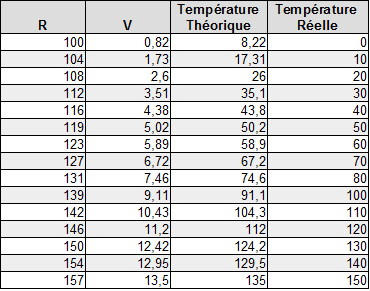
\includegraphics[width=12cm]{../Images/TabPT100.png}
			\end{center}

      \par Ces données nous permettent de tracer les courbes suivantes, comparant les valeurs de température théorique et celle fourni par la documentation de la PT100 :
			\begin{center}
				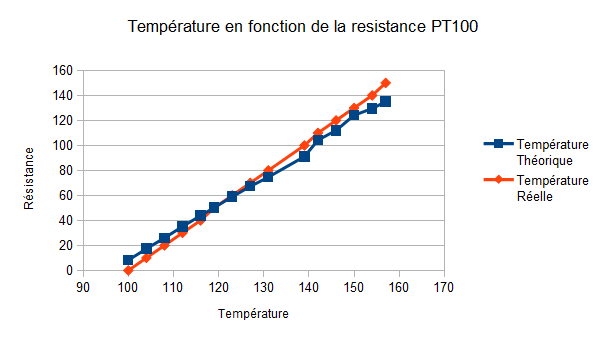
\includegraphics[width=12cm]{../Images/GraphPT100.png}
			\end{center}
    \newpage

  \section{Thermocouple}
		\subsection{Réglage de la compensation}
			\par Avant de connecter le thermocouple, nous réglons la tension de compensation à l'aide du potentiomètre P3 de sorte à compenser la température ambiante et obtenir les valeurs disponibles sur la table du thermocouple type J pour cette valeur de température. Pour mesurer cette tension, nous connectons le voltmètre au niveau de la borne VE-.

		\subsection{Réglage du gain}
			\par Afin d'obtenir les valeurs souhaitées avec le thermocouple, nous le branchons sur la plaquette en faisant attention au sens du branchement (Fil blanc sur VE- et noir sur VE+). Ensuite nous mesurons la tension au niveau de la sortie devant posséder une sensibilité de 10 mV/{\degre}C et réglons le gain à l'aide du potentiomètre P4 afin d'obtenir effectivement cette sensibilité.

		\subsection{Mesures}
			\par Nous obtenons ainsi que le thermocouple fonctionne et avons testé son fonctionnement en mesurant la température d'un glaçon, la température ambiante et la température du corps humain.
      		\begin{itemize}
				\item Corps humain: 0.3 V
				\item Glace: 0.092 V
				\item ambiante: 0.226 V
			\end{itemize}

  \section{Capteur de type NTC}
  		\subsection{Réglage du zéro}
			\par Afin d'utiliser la sonde NTC il est nécessaire tout d'abord de régler le zéro. Pour cela nous plaçons les cavaliers de la manière suivante:
      		\begin{itemize}
				\item Pour C1, nous relions les bornes 1 et 3.
				\item Nous relions les bornes de C2.
				\item Nous ne relions pas les bornes de C3.
			\end{itemize}
			\par On connecte ensuite une résistance variable entre RNTC1 et RNTC2, on la met à la valeur de la résistance NTC à 0{\degre}C, puis on règle le potentiomètre de réglage du zéro de sorte à obtenir VOUT = 0 V.

		\subsection{Réglage du gain}
			\par L'étape qui vient ensuite est le réglage du gain. Pour cela nous réglons la résistance variable à la valeur de résistance de la sonde NTC à 25{\degre}C et on règle le potentiomètre de gain de sorte à obtenir une sensibilité de 100mV/{\degre}C.

		\subsection{Simulation}
			\par On fait une simulation des températures qu'on devrait obtenir en utilisant différentes valeurs de résistance à la place du capteur NTC.
			On obtient le tableau de données suivant:
			\begin{center}
				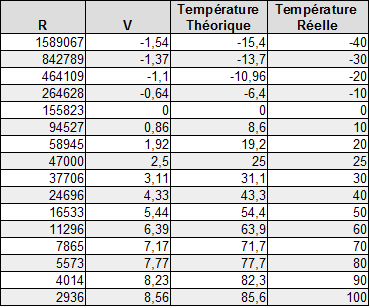
\includegraphics[width=12cm]{../Images/TabNTC.png}
			\end{center}

			\par Ces données nous permettent de tracer les courbes suivantes, comparant les valeurs de température théorique et celle fourni par la documentation du capteur NTC :
			\begin{center}
				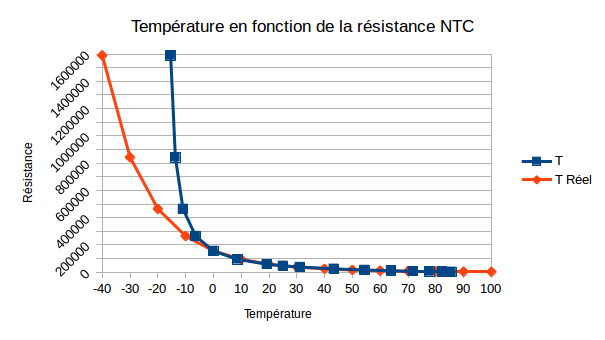
\includegraphics[width=12cm]{../Images/GraphNTC.png}
			\end{center}
			\par On constate une nette différence entre les valeurs attendues et les valeurs obtenues lorsque les températures sont basses.

	\section{Conclusion}
	\label{sec:Conclusion}
		\par Le type de capteur utilisé dépend fortement de l'utilisation que l'on souhaite en faire.
		En effet, nous avons constaté durant ce TP que ces capteurs avaient des précisions et des vitesses de transition différentes:
		\par La sonde PT100 possède une grande rapidité de réponse aux changements thermiques tout en étant précise face aux températures de notre environnement.
		\par Le capteur NTC est quant à lui beaucoup moins précis, mais possède l'avantage de pouvoir supporter une plage de température bien plus importante.

\end{document}
